\documentclass[tikz, border=10pt]{standalone}
\usepackage{tkz-euclide}

\begin{document}
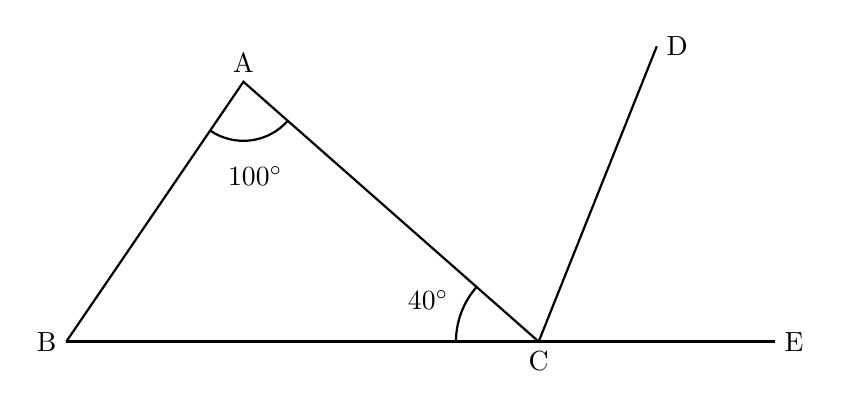
\begin{tikzpicture}[scale=1.5]
    % --- Coordinates ---
    \coordinate (B) at (0,0);
    \coordinate (C) at (4,0);
    \coordinate (E) at (6,0);
    \coordinate (A) at (1.5,2.2);
    \coordinate (D) at (5,2.5);

    % --- Lines ---
    \draw[thick] (B) -- (E);        % Straight baseline BE
    \draw[thick] (B) -- (A) -- (C); % Triangle sides
    \draw[thick] (C) -- (D);        % Ray CD

    % --- Points Labels ---
    \node[left] at (B) {B};
    \node[below] at (C) {C};
    \node[right] at (E) {E};
    \node[above] at (A) {A};
    \node[right] at (D) {D};

    % --- FIXED Angle 100 at A using tkz-euclide ---
    % This automatically calculates the intersection with lines AB and AC
    \tkzMarkAngle[size=0.5, thick](B,A,C)
    \tkzLabelAngle[pos=0.8](B,A,C){$100^\circ$}

    % --- FIXED Angle 40 at C using tkz-euclide ---
    % This automatically calculates the intersection with lines AC and CB
    \tkzMarkAngle[size=0.7, thick](A,C,B)
    \tkzLabelAngle[pos=1.0](A,C,B){$40^\circ$}

\end{tikzpicture}
\end{document}
